\documentclass{standalone}
\usepackage{standalone}

\begin{document}
\chapter{Data Sets}
This section will introduce to our collected dataset in brief. 

\subsection{Variety of Images}
An image of a car can vary in many ways. Here are some of possible reason for variance:
\begin{itemize}
    \item Positions of plate varies in cars to cars.
    \item Colors of plates are different in many cars.
    \item Non-standard use of fonts.
    \item Materials of plates.
    \item Muds on license plate.
    \item Erased characters on plates.
    \item Due to the conditions of weather and time of the day, the light may prove a significant factor of variance. 
    \item The sun may create reflection on the license plates.
    \item Due to bumper-guards, the plate may be hidden in some cars.
    \item Image size may vary depending on the camera type.
    \item Resolution of the image taken may vary.
    \item Types and colors of plate puts an effect in plate image.
\end{itemize}

\subsection{Collected Dataset}
Due to the different conditions it is very difficult to collect a good enough data sets to properly capture all conditions. The conditions and variety of our dataset is represent in Table \ref{table:Variety}. Note that, same image fall into more than one category in the table below and the count was done in that way. 

\begin{table}    
    \caption{Data-set for experimentation}
    \label{table:Variety}
    \begin{tabular}{|l|r|}
    \hline
    {\bf Variety}  &  {\bf Number Of Images} \\ 
    \hline 
    In good condition &  42 \\ 
    Highly angled/skewed plate & 16 \\
    Bad Resolution & 19 \\ 
    Non-Standard Plates &  18\\    
    Private Vehicle & 8 \\
    Shadowed license plate & 11 \\    
    Light reflection & 9 \\
    Small plates & 6\\
    Muddy, erased or hidden letters & 18 \\
    Unrecognizable plates (for the bumper, mud, light etc.) & 14  \\
    \hline
    {\bf Total plates} & {\bf 138} \\
    \hline
    \end{tabular}
\end{table}

In our experimentation, we did not keep Unrecognizable plate images, and removed some bad quality images. Our final dataset was consists of $78$ images of different categories.

\subsection{Image samples}
Some sample images we used during our experimentation are shown in following figures.

\begin{figure}
\begin{subfigure}{0.5\textwidth}
    \centering
    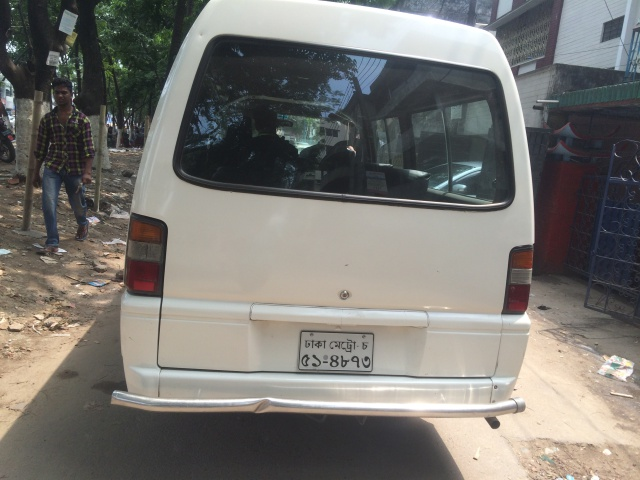
\includegraphics[width=0.9\linewidth]{./img/experiment/stage.1/angle}
\end{subfigure}
\begin{subfigure}{0.5\textwidth}
    \centering
    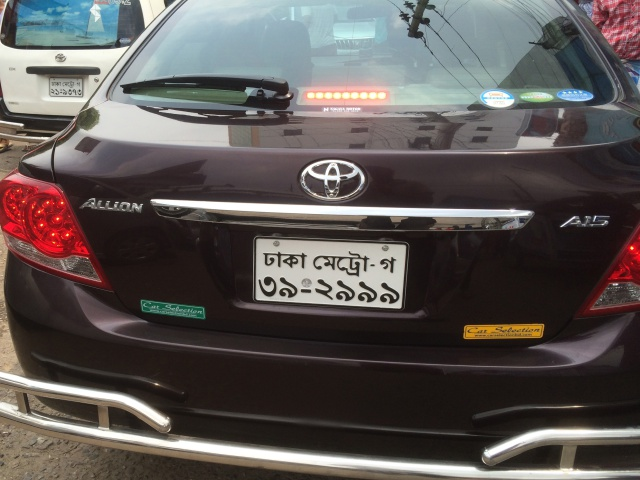
\includegraphics[width=0.9\linewidth]{./img/experiment/stage.1/angle3}
\end{subfigure}
\caption{Slightly angled license plates}
\end{figure}

\begin{figure}
    \centering
    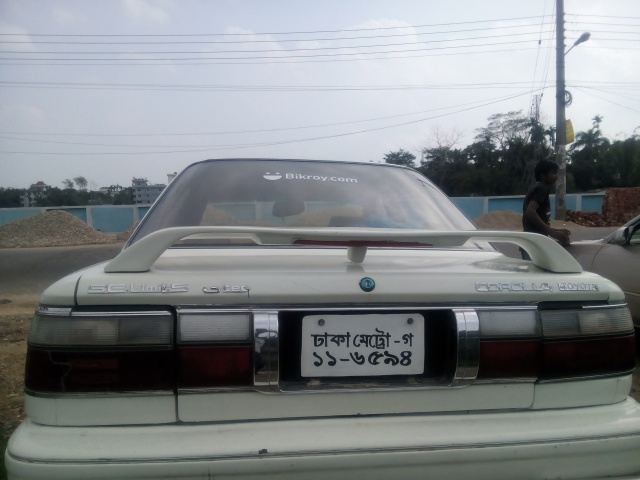
\includegraphics[width=0.5\textwidth]{./img/experiment/stage.1/badfont}
    \caption{Non-standard use of font}
\end{figure}

\begin{figure}
    \centering
    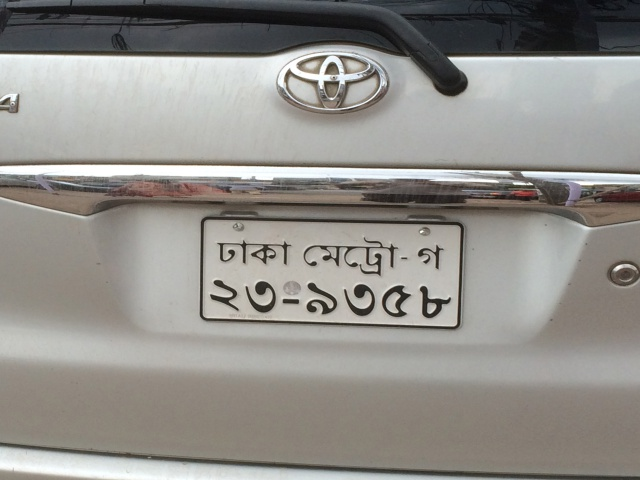
\includegraphics[width=0.5\textwidth]{./img/experiment/stage.1/big}
    \caption{Closed focus}
\end{figure}

\begin{figure}
    \centering
    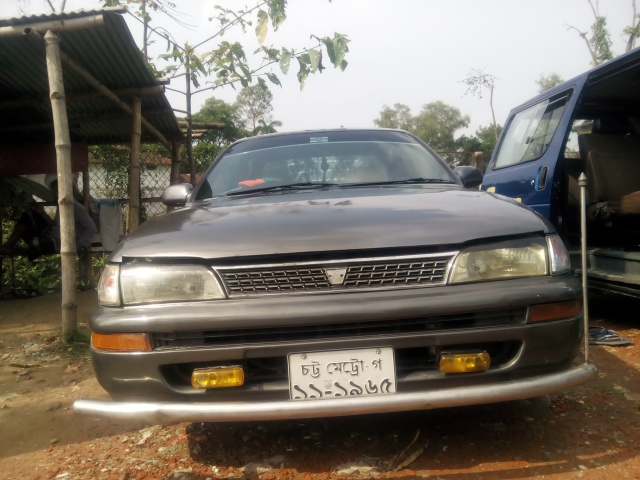
\includegraphics[width=0.5\textwidth]{./img/experiment/stage.1/bumper}
    \caption{Bumper hides a part of plate}
\end{figure}

\begin{figure}
    \centering
    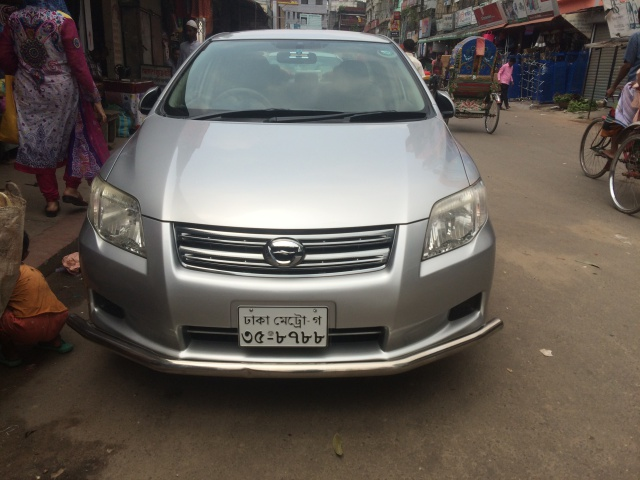
\includegraphics[width=0.5\textwidth]{./img/experiment/stage.1/good}
    \caption{The camera is not focused on the plate}
\end{figure}

\begin{figure}
\begin{subfigure}{0.5\textwidth}
    \centering
    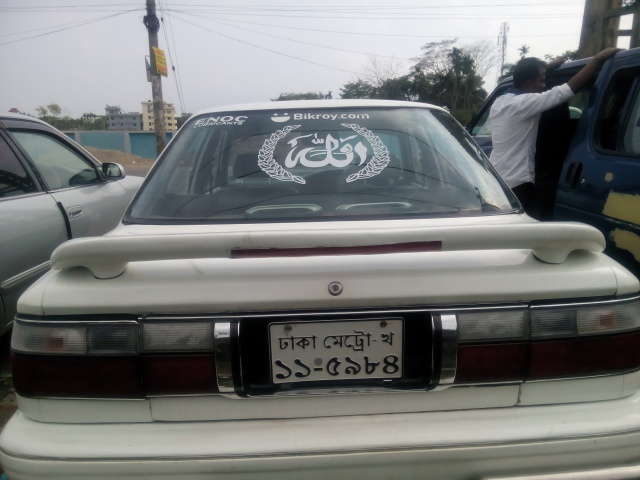
\includegraphics[width=0.9\linewidth]{./img/experiment/stage.1/good2}
\end{subfigure}
\begin{subfigure}{0.5\textwidth}
    \centering
    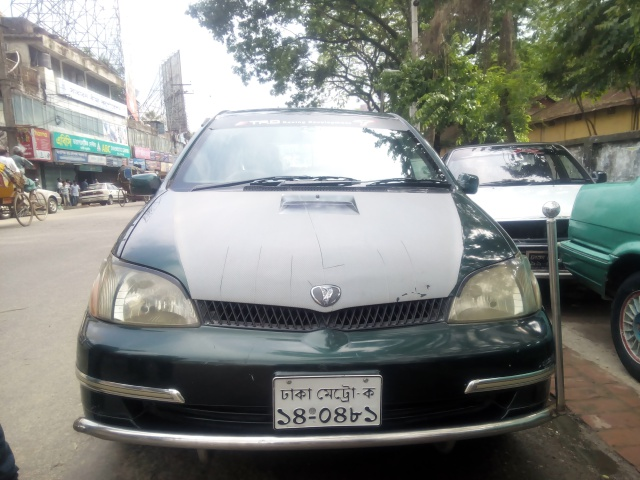
\includegraphics[width=0.9\linewidth]{./img/experiment/stage.1/good3}
\end{subfigure}
\caption{Moderate quality images}
\end{figure}


\begin{figure}
\begin{subfigure}{0.5\textwidth}
    \centering
    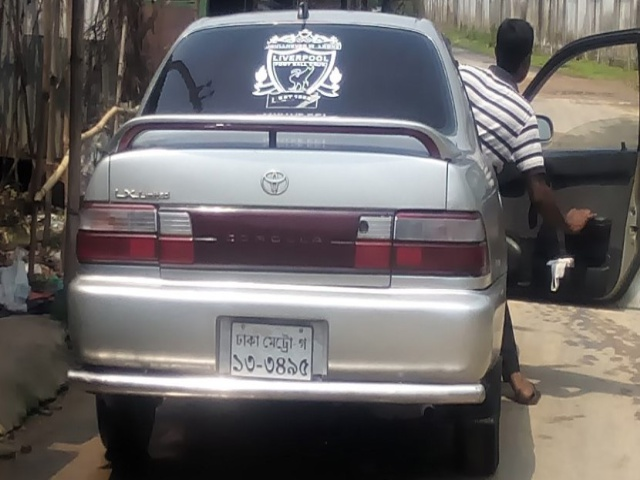
\includegraphics[width=0.9\linewidth]{./img/experiment/stage.1/light}
    \caption{On Plate}
\end{subfigure}
\begin{subfigure}{0.5\textwidth}
    \centering
    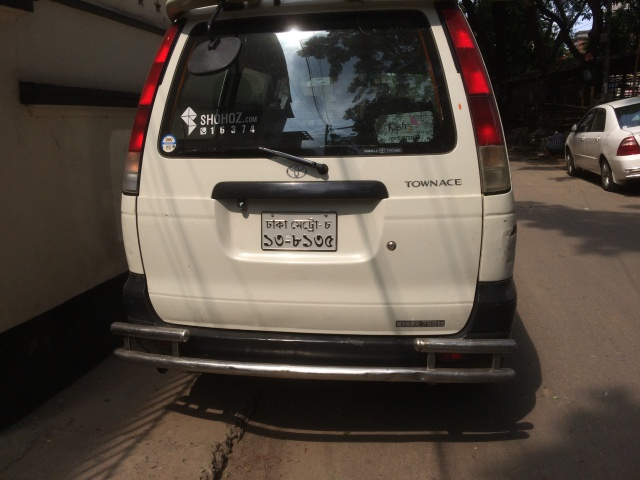
\includegraphics[width=0.9\linewidth]{./img/experiment/stage.1/light2}
    \caption{On Text}
\end{subfigure}
\caption{Reflection of light}
\end{figure}

\begin{figure}
\begin{subfigure}{0.5\textwidth}
    \centering
    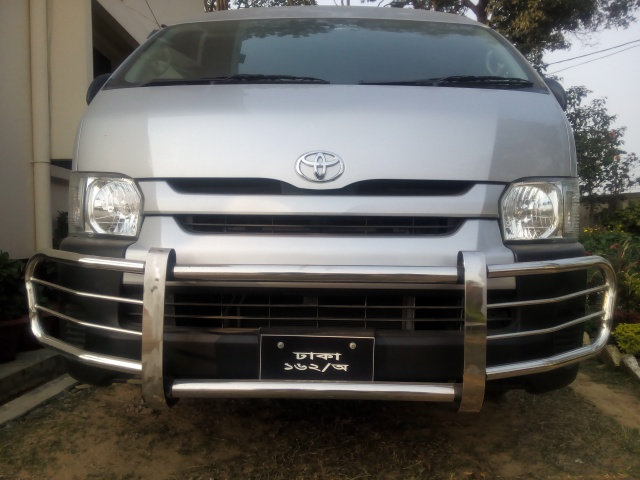
\includegraphics[width=0.9\linewidth]{./img/experiment/stage.1/nostd2}
    \caption{Private plate}
\end{subfigure}
\begin{subfigure}{0.5\textwidth}
    \centering
    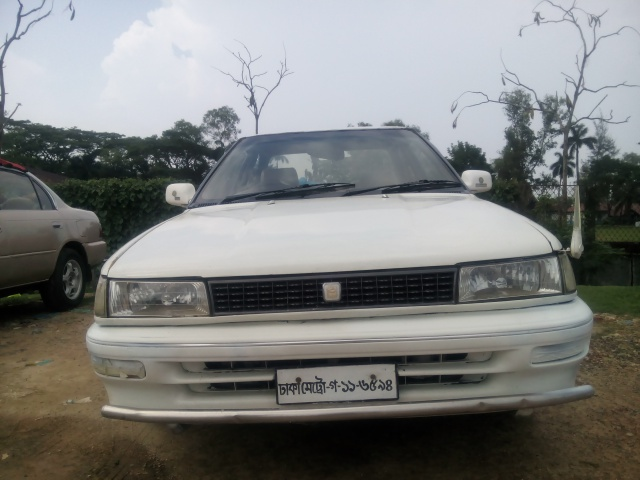
\includegraphics[width=0.9\linewidth]{./img/experiment/stage.1/nostd}
    \caption{One-line}
\end{subfigure}
\caption{Non-standard license plate}
\end{figure}

\begin{figure}
\begin{subfigure}{0.5\textwidth}
    \centering
    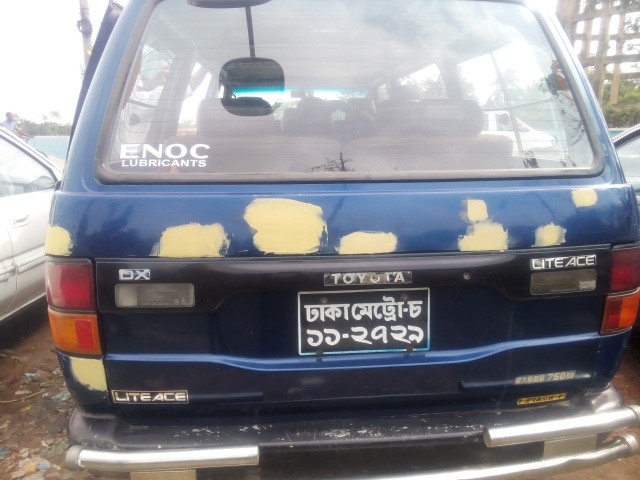
\includegraphics[width=0.9\linewidth]{./img/experiment/stage.1/private}
    \caption{Noisy}
\end{subfigure}
\begin{subfigure}{0.5\textwidth}
    \centering
    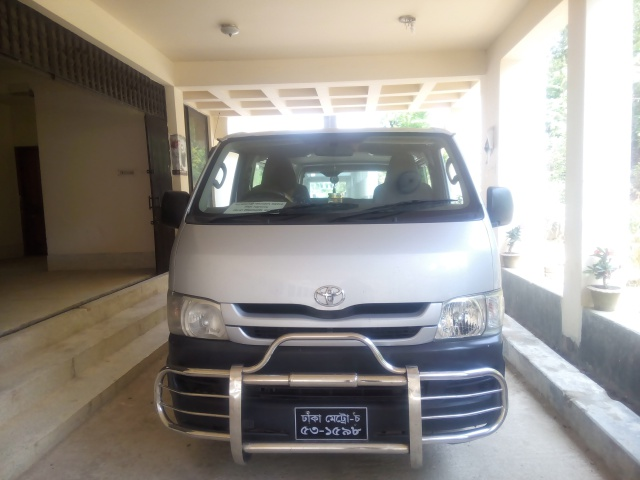
\includegraphics[width=0.9\linewidth]{./img/experiment/stage.1/private2}
    \caption{Good}
\end{subfigure}
\caption{Private plate (white text on black plate).}
\end{figure}


\begin{figure}
    \centering
    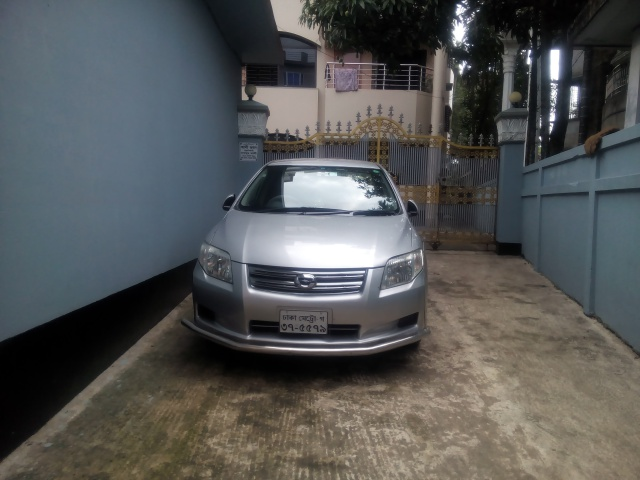
\includegraphics[width=0.8\textwidth]{./img/experiment/stage.1/small}
    \caption{Small plate (Camera is far from the car).)}
\end{figure}

\end{document}